 %!TEX root = ./template-skripsi.tex
%-------------------------------------------------------------------------------
%                            BAB II
%               KAJIAN TEORI
%-------------------------------------------------------------------------------

\chapter{KAJIAN PUSTAKA} 

\section{Konsep Budidaya Ikan Air Tawar}

Budidaya adalah kegiatan  memproduksi dan mengembangkan biota (organisme) dalam lingkungan yang terkendali untuk mendapatkan keuntungan. Budidaya ikan air tawar merupakan kegiatan yang dilakukan untuk meningkatkan produktivitas perairan,  khususnya ikan air tawar. Kegiatan budidaya dimaksudkan untuk memperbanyak, menumbuhkan dan meningkatkan kualitas biota perairan itu sendiri untuk menghasilkan keuntungan. Sementara budidaya perikanan modern merupakan metode budidaya yang menggabungkan teknologi terbaru dan ilmu pengetahuan untuk menciptakan lingkungan yang optimal bagi pertumbuhan dan kesehatan ikan \citep{bangkit2016}.

Akuakultur (budidaya ikan) merupakan salah satu subsektor yang diharapkan dapat mewujudkan misi mensejahterakan perikanan. Akuakultur tingkat rendah berkontribusi pada kesejahteraan petani ikan untuk menjamin ketersediaan pangan, gizi dan kesehatan di daerah. Budidaya perikanan modern menggunakan pelet dan konsetrat sebagai sumber pakan, selain itu juga diterapkan berbagai treatment kedalam sistem budidaya untuk membantu proses budidaya ikan. Contoh metode budidaya perikanan modern yaitu RAS dan Biofloc.  


\section{\textit{Food Conversion Ratio (FCR)}}
FCR (Feed Conversion Ratio) pada budidaya ikan adalah suatu ukuran yang menyatakan rasio jumlah pakan yang dibutuhkan untuk menghasilkan 1 kg daging ikan. FCR juga sering digunakan untuk mengetahui kualitas pakan yang diberikan terhadap pertumbuhan ikan. Informasi mengenai FCR ikan yang dibudidayakan sangat penting karena berkaitan dengan efisiensi pakan dan efisiensi musim budidaya. Menurut \citep{effendie1997} FCR ikan didapatkan melalui rumus berikut.

\begin{equation*}
	FCR=\frac{Berat Total Ikan Panen(Kg)}{Jumlah Pakan(Kg)}
\end{equation*}

Informasi mengenai FCR ikan yang dibudidayakan sangat penting karena berkaitan dengan efisiensi pakan. Efisiensi pakan berfungsi mengukur tingkat penggunaan input, yakni pakan dan output berupa bobot daging ikan. Semakin kecil nilai efisiensi pakan, berarti pakan yang diberikan sudah baik. Efisiensi pakan berhubungan dengan pertambahan berat, konsumsi pakan, dan konversi pakan. Pertambahan berat dapat dihitung dengan mengurangi bobot badan ikan saat panen dengan bobot ikan pada awal penebaran.

Sementara itu, konversi pakan merupakan pembagian antara berat badan yang dicapai pada bulan berlangsung dengan konsumsi pakan pada bulan tersebut. Konversi pakan didapatkan dengan membagi total pakan yang dikonsumsi dengan total hasil produksi.

Efisiensi berkaitan erat dengan biaya yang harus Anda keluarkan selama budidaya. Apabila efisiensi pakan tidak bagus, kemungkinan besar biaya pakan yang dikeluarkan juga besar. Padahal, pakan merupakan komponen penting dan besar dalam usaha budidaya. Semakin besar biaya pakan, akan semakin besar juga biaya produksi yang dibutuhkan.

\section{\emph{Recirculating aquaculture system (RAS)}}

RAS merupakan sistem budidaya yang menggunakan air daur ulang yang pertama kali diperkenalkan di Amerika Serikat pada awal tahun 1960 dan mulai diterapkan sejak tahun 1990-an. Teknologi RAS pada saat itu menjadi solusi atas permasalahan pencemaran organik sungai dari tempat budidaya bersamaan dengan permintaan benih ikan salmon yang tinggi yang dibutuhkan sepanjang waktu (kontinu). Kualitas suatu perairan merupakan syarat penting yang dapat mempengaruhi kelangsungan hidup perkembangan, pertumbuhan, dan tingkat produksi ikan. Lingkungan yang baik sangat diperlukan untuk kelangsungan hidup organisme akuatik. Sistem ini telah banyak dikembangkan dan iterapkan dibeberapa negara maju, seperti Amerika, Israel, Singapura, German serta Norwegia selama kurun waktu 20-30 tahun ini \citep{fadhil2010}.

Teknologi RAS menawarkan sebuah alternatif teknologi budidaya melalui perbaikan kualitas air dan penggunaan kembali (re-use). Penggunaan RAS secara intensif terbukti dapat mengurangi secara signifikan konsumsi air dan konsentrasi nutrien melalui perbaikan dan pengembangan teknologi secara berkelanjutan \citep{thesiana2015}. RAS dapat digunakan untuk mengontrol beberapa parameter kualitas air penting seperti oksigen terlarut, karbondioksida, amonia, nitrit, nitrat, pH, salinitas, dan padatan tersuspensi. Hal ini memungkinkan terciptanya kondisi pemeliharaan yang baik untuk pertumbuhan dan pemanfaatan pakan yang lebih optimal \citep{dalsgaard2013}.

\section{\emph{Biofloc Technology}}

Teknologi bioflok merupakan teknologi penggunaan bakteri baik heterotrof maupun autotrof yang dapat mengonversi limbah organik secara intensif menjadi kumpulan mikroorganisme yang berbentuk flok, kemudian dapat dimanfaatkan oleh ikan sebagai sumber makanan. Di dalam flok terdapat beberapa organisme pembentuk seperti bakteri, plankton, jamur, alga, dan partikel tersuspensi yang memengaruhi struktur dan kandungan nutrisi bioflok, namun komunitas bakteri merupakan mikroorganisme paling dominan dalam pembentukan flok dalam bioflok. 

Agregat bioflok memiliki rentang ukuran partikel yang luas, mulai dari yang mikroskopis hingga yang lebih besar dari 1 mm. Bahkan organisme yang lebih besar seperti copepoda dan nematoda dapat memakan flok dan menjadi bagian yang tidak terpisahkan dari beberapa agregat. Kepadatan flok dengan berat basah biasanya hanya sedikit lebih besar dari 1 g/mL, jadi agregat akan tenggelam perlahan-lahan dan relatif mudah dipelihara suspensinya. Dengan porositas hingga 99 persen (ruang kosong), nutrisi, oksigen, dan produk limbah mudah dipertukarkan di antara bagian dalam flok dan air di sekitarnya, dan ini ditingkatkan oleh pencampuran umum dalam sistem bioflok\citep{samocha2019}.

Mikroorganisme bioflok bervariasi antar sistem dan juga dalam sistem yang sama dari waktu ke waktu mengidentifikasi fluktuasi dalam komposisi taksonomi bakteri, mikroalga, ragi, dan mikroorganisme lain dalam flok dari sistem bioflok ikan nila. Di antara bakteri dan ragi taksa adalah Aeromonas spp., Vibrio spp., Enterobac ter sp., Nitrospira sp., Bacillus spp., Sphingomonas sp., Pseudomonas spp., Microthrix sp., Nitrobacter sp., Micrococcus sp., Alcaligenes sp., dan Rhodotorula sp. Bakteri biasanya mendominasi bioflok di sistem akuakultur. Tidak hanya berlimpah (hingga 100 juta bakteri/mL), tetapi juga menunjukkan keragaman yang tinggi. terdapat gambaran menyeluruh pembahasan banyak faktor yang menentukan komposisi flok, diantaranya adalah suhu, salinitas, pH, penyinaran, intensitas pencampuran vertikal, dan jenis karbon organik yang tersedia untuk metabolisme bakteri.

Laju perkembangan flok bisa ditingkatkan dengan cara menambahkan organik karbon untuk merangsang pembentukan flok. Perkembangan dipengaruhi oleh berbagai faktor, yang terutama adalah suhu, oksigen terlarut, pH, beban organik, cahaya, dan pencampuran. \citep{samocha2019} juga menjelaskan mengenai faktor-faktor tersebut:

\begin{enumerate}
	\item Agregat lebih besar dan lebih padat di tempat yang suhunya lebih tinggi dan oksigen terlarut lebih tinggi.
	\item Pencampuran yang intens mengganggu agregat dan mengurangi ukuran flok rata-rata.
	\item Laju pemompaan tinggi melalui lubang kecil mengurangi ukuran flok.
	\item Oksigen terlarut lebih rendah mendukung filamen bakteri, kemungkinan karena rasio permukaan-ke-volume yang tinggi.
	\item pH mempengaruhi flok secara langsung, setiap spesies memiliki range pH opminal masing masing dan berhubungan langsung dengan alkalinitas, karbon anorganik, dan amonia.
	\item Muatan organik tinggi berpromosi lebih cepat berkembang.
	\item Cahaya mempengaruhi kelimpahan organisme fotoautotrofik (yaitu, cyanobacteria, ganggang hijau, diatom, dinoflagellata, rhodophyta, dll.) dalam flok.
\end{enumerate}

Di antara keunggulan bioflok dalam akuakultur adalah nilai nutrisinya yang tinggi, perannya dalam meningkatkan kualitas air, dan efek probiotiknya pada ikan:
\begin{enumerate}
	\item Bioflok sebagai pakan

	Bioflok memiliki kualitas nutrisi yang mirip dengan makanan yang dimakan ikan liar di habitat alaminya. Mempertahankan kepadatan flok yang sesuai di seluruh siklus tanaman dapat mengurangi kebutuhan akan pakan yang diformulasikan \citep{avnimelech2009} yang biasanya menyumbang setidaknya setengah dari biaya produksi dalam akuakultur tradisional. Kuantitas dan kualitas bahan organik disimpan oleh bakteri akhirnya menentukan nilai gizi flok. Bahan organik yang disimpan ini tergantung pada jumlah dan jenis organik karbon yang tersedia untuk pertumbuhan bakteri. intinya adalah bahwa "bioflok adalah apa yang dimakannya". Jika substrat organik yang tepat disediakan, kemudian floc akan menyimpan senyawa berkualitas tinggi itu, maka hal tersebut akan berkontribusi terhadap kebutuhan nutrisi ikan.

	\item Bioflok dan kualitas air

	Di luar nilai nutrisinya, bakteri bioflok dapat dikelola untuk meningkatkan kualitas air. Ini dapat diklasifikasikan menurut caranya memperoleh yaitu, autotrof dan heterotrof. Baik organisme autotrofik dan heterotrofik yang mengisi agregat bioflok meningkatkan kualitas air dengan asimilasi atau transformasi senyawa nitrogen anorganik terlarut (amonia, nitrit, nitrat) yang berbeda derajat, hal ini berbahaya bagi ikan. Untuk tujuan ini, sistem yang didominasi bioflok dapat dikelola mendukung bakteri autotrofik, bakteri heterotrofik, atau kombinasi keduanya dalam sistem mixotrophic. Setiap pilihan memiliki perbedaan implikasi terhadap kualitas air.

	\item Bioflok dan respon immune

	Beberapa jenis ikan memiliki sistem kekebalan yang labil. Ini berarti bahwa mereka tidak memiliki antibodi-antigen spesifik mekanisme untuk menanggapi patogen baru. Populasi mikroba dalam sistem bioflok, Namun, mungkin berperan dalam mengaktifkan sistem kekebalan non spesifik mereka, menghasilkan pertahanan
\end{enumerate}

Pada sistem akuakultur dengan teknologi bioflok, air media kultur hanya sekali dimasukkan dalam wadah, dan digunakkan sampai panen. Penambahan air hanya untuk pengganti penguapan dan pengontrolan kepadatan bioflok \citep{avnimelech2009}. Dibanding sistem resirkulasi yang sangat kompleks, sistem kultur dengan teknologi bioflok hanya menggunakan satu wadah, yakni wadah kultur. Penguraian bahan organik oleh bakteri dan mikroorganisme pengurai, sampai pada pemanfaatan hasil penguraian oleh mikroalga dan mikroorganisme yang tumbuh, terjadi dalam wadah secara seimbang dengan kepadatan organisme kultur yang sangat tinggi. Pengontrolan kualitas air terjadi dalam wadah kultur itu sendiri, oleh sistem bioflok yang sudah berjalan dalam wadah kultur. Sistem ini sangat murah, sederhana ramah lingkungan dan memiliki produktifitas yang sangat tinggi \citep{taw2012}.

\section{Front-end dan Back-End}

Frontend adalah bagian yang dilihat dan dilihat oleh pengguna untuk berinteraksi dengannya, seperti menu, formulir kontak, dll. Dalam konteks web, front end dibuat dengan menggunakan HyperText Markup Language (HTTP), Cascading Style Sheets (CSS), dan juga JavaScript. Sehingga, suatu URL bisa bekerja dan menampilkan situs website dengan baik. Sementara dalam aplikasi mobile, front end dibuat dengan menggunakan widget untuk menampilkan suatu fitur untuk berkomunikasi dengan pengguna. Oleh karena itu, front end juga bisa disebut sebgai client-side.

Di sisi lain, backend biasanya terdiri dari tiga bagian: server, aplikasi, dan DB. Bagian belakang teknologi biasanya terdiri dari bahasa seperti PHP, Ruby, Python, dll. Pada bagian back end, semua hal yang dibuat di dalam front end ataupun sistem dan server dibalik dibuatnya situs website atau aplikasi bisa bekerja sebagaimana mestinya. Mereka juga sering disebut dengan server-side.

\section{Dart}

Bahasa pemrograman Dart merupakan bahasa pemrograman general-purpose yang dirancang oleh Lars Bak dan Kasper Lund. Bahasa pemrograman ini dikembangkan sebagai bahasa pemrograman aplikasi yang dapat dengan mudah untuk dipelajari dan disebarkan. Bahasa pemrograman Dart dapat digunakan secara bebas oleh para developer, karena bahasa ini dirilis secara open-source oleh Google di bawah lisensi BSD. Bahasa pemrograman Dart merupakan bahasa pemrograman berbasis class dan berorientasi terhadap obyek dengan menggunakan sintaks bahasa pemrograman \citep{kelvin2021}. Berikut adalah contoh program sederahana dari Dart guna lebih memahami bahasa pemrograman tersebut:

\begin{enumerate}
	\item \textit{Main Function}

	Setiap aplikasi mempunyai Main Fuction, berikut adalah contoh Main Function yang akan menampilkan teks pada console. Untuk menerapkannya, bisa digunakan print() function.
	
	\begin{figure}[H]
		\centering
		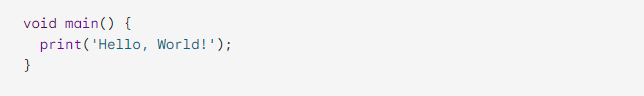
\includegraphics[keepaspectratio, width=12cm]{gambar/helloworld}
		\caption{Contoh Main Function}
		\label{gambar:main}
	\end{figure}
	
	\item Deklarasi \textit{Variables}

	Berikut adalah contoh deklarasi Variable pada dart:
	\begin{figure}[H]
		\centering
		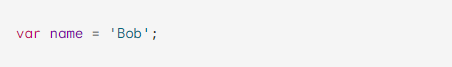
\includegraphics[keepaspectratio, width=12cm]{gambar/implisitvar}
		\caption{Contoh Deklarasi Variable}
		\label{gambar:deklarasivariable}
	\end{figure}
	Pada gambar 2.2 dapat diketahui bahwa terdapat variable yang bernama name dengan bentuk String bernilai "Bob". Variable akan disimpulkan secara implisit dalam bentuk String meskiput tidak dideklarasi secara eksplisit, namun jika dibutuhkan untuk mendeklarasikan variabel secara eksplisit, maka menggunakan cara deklarasi secara eksplisit seperti pada gambar 2.3.
	\begin{figure}[H]
		\centering
		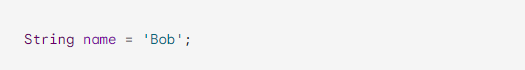
\includegraphics[keepaspectratio, width=12cm]{gambar/eksplisitvar}
		\caption{Contoh Deklarasi Variabel Secara Eksplisi}
		\label{gambar:deklarasivariableeksplisit}
	\end{figure}
	
	\item\textit{Classes}

	Dart adalah bahasa berorientasi objek dengan Class dan pewarisan berbasis mixin. Setiap objek adalah turunan dari Class, dan semua Class kecuali Null turun dari Objek. Pewarisan berbasis mixin berarti meskipun setiap Class (kecuali Top-Class) memiliki tepat satu superclass, Class dapat digunakan kembali dalam beberapa hierarki Class. Metode Extendsi adalah cara untuk menambahkan fungsionalitas ke Class tanpa mengubah Class atau membuat subclass. Dapat Dilihat pada gambar 2.4 yaitu contoh sebuah Class pada bahasa pemrogramman Dart.
	\begin{figure}[H]
		\centering
		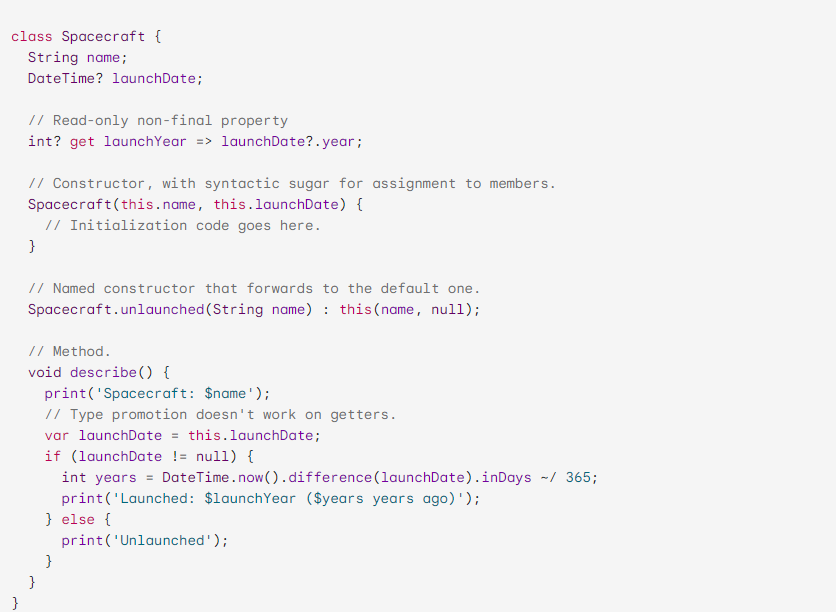
\includegraphics[keepaspectratio, width=9cm]{gambar/Classes}
		\caption{Contoh Class Pada Dart}
		\label{gambar:Class}
	\end{figure}

\end{enumerate}


\section{Flutter}

Flutter telah diresmikan sejak tahun 2015 oleh developer Dart yaitu Sky. Eric Seidel (Direktur untuk Flutter diGoogle). Flutter adalah cross-platform framework yang dibuat oleh Google untuk membangun berbagai aplikasi seperti android mobile, iOS mobile, web, dan desktop. sedangkan menurut \citep{napoli2019} Flutter adalah kerangka antarmuka pengguna portabel (UI) Google untuk membangun aplikasi modern, asli, dan reaktif untuk iOS dan Android. Framework ini menggunakan widgets untuk membuat UI dan Dart sebagai bahasa pemograman untuk mengembangkan aplikasinya. Widget dapat diibaratkan dengan permainan Lego yang bisa menambahkan berbagai macam jenis bongkahan plastik kecil dan mengubah tampilan UI sesuai dengan yang diinginkan oleh developer.

Flutter mempunyai dua macam widget untuk pengembang aplikasi pakai, yaitu Material Design dan Cupertino. Material Design adalah bahasa design yang dibuat oleh Google, design ini sama dengan design yang dipakai pada Android. Cupertino atau dengan sebutan lain gaya iOS adalah bahasa design yang dipakai oleh iOS. Flutter mempunyai lebih banyak widget Material Design daripada widget Cupertino, walaupun demikian, pada OS perangkat yang berbeda, widget bisa dipakai secara cross platform. Flutter memiliki berbagai macam keuntungan dibanding framework lain diantaranya:


\begin{enumerate}
	\item Tingkatkan produktivitas

	Dalam mengembangkan aplikasi berbasis Android dan iOS, Anda hanya membutuhkan satu basis kode. Ini membuat Anda lebih menghemat waktu dan tim.
	
	\item Tingkatkan produktivitas

	Tampilan desain yang sangat bagus. Flutter menyediakan widget cantik yang dapat disesuaikan dengan mudah untuk membuat aplikasi terlihat lebih menarik. Jadi, dengan menggunakan Flutter, developer dari setiap level keahlian akan lebih mudah membuat aplikasi terlihat lebih baik.

	\item Mudah untuk dipelajari

	Flutter adalah framework yang mudah dipelajari. Selain itu, Flutter juga memungkinkan developer aplikasi untuk membangun aplikasi tanpa menggunakan banyak kode seperti pada framework lainnya.

	\item Performa kerangka kerja yang hebat

	\item Pembuatan hemat biaya

	Membuat dua aplikasi (Android dan iOS) dengan menggunakan satu codebase tentunya dapat lebih menghemat biaya pengembangan aplikasi.

	\item Tersedia dalam berbagai pilihan aplikasi IDE (Integrated Development Environment)

	Anda dapat memilih untuk mengembangkan aplikasi (Flutter) menggunakan Android Studio, atau dengan VS Code.

	\item Dokumentasi lengkap dan komunitas aktif.

	Anda dapat membuka dokumentasi melalui situs resmi Flutter. Selain itu, Anda juga bisa bergabung dengan komunitas untuk berdiskusi dengan sesama pengguna Flutter.

\end{enumerate}


\section{Flutter Widget}

Flutter menggunakan konsep widget untuk membuat tampilannya. Widget adalah komponen UI yang membangun aplikasi Flutter. Setiap membuat UI dalam Flutter akan menciptakan berbagai macam pohon widgets . Berikut beberapa informasi mengenai widget:
\begin{enumerate}
	\item Widget digunakan untuk membuat UI, seperti: baris, kolom, stack, card, form, dan padding.
	\item Pada Widget, developer dapat melakukan styling, seperti: tipe font, ukuran, berat, warna, batas, dan bayangan. 
	\item Widget dapat berupa kumpulan bentuk dan formulir.
\end{enumerate}

Diantara widget-widget tersebut, ada beberapa widget yang sering digunakan dan diterapkan dalam berbagai macam aplikasi seperti: CardView, PageView, Bottom Navigation View. Untuk mengetahui lebih lanjut tentang wdget-widget pada flutter.

\section{Metode Scrum}
Metode Scrum diciptakan oleh Jeff Sutherland dan tim pengembangnya pada awal 1990-an. Sutherland, Viktorov, Blount dan Puntikov menggambarkan Scrum sebagai “Proses pengembangan perangkat lunak \textit{Agile} yang dirancang untuk menambah energi, fokus, kejelasan, dan transparansi bagi tim proyek yang mengembangkan sistem perangkat lunak” \citep{sutherland2007}. Proses Scrum mematuhi prinsip-prinsip pendekatan \textit{Agile}. Prinsip pendekatan \textit{Agile} berfokus pada memuaskan pelanggan melalui pengiriman awal perangkat lunak yang berharga; membolehkan perubahan kebutuhan; kolaborasi antara pengembang dan pelaku bisnis; perangkat lunak yang berfungsi (sebagai ukuran kemajuan); menjaga desain tetap sederhana; dan secara berkala, membuat tim merenungkan bagaimana menjadi lebih efektif selama proses pengembangan.

Scrum menawarkan cara yang dapat disesuaikan untuk bekerja pada proyek yang berbeda yang memiliki berbagai persyaratan dan Scrum memiliki keunggulan seperti pemilihan persyaratan atau spesifikasi kebutuhan yang fleksibel untuk \textit{sprint} dan tidak ada prosedur khusus yang harus diikuti. Prinsipnya adalah bekerja secara iteratif hingga mencapai waktu yang ditentukan dan dapat memenuhi kebutuhan konsumen. Scrum menerapkan metode ilmiah empirisme. Scrum 
menggantikan pendekatan algoritmik terprogram dengan pendekatan heuristik, dengan menghormati orang dan pengaturan diri untuk menghadapi ketidakpastian dan memecahkan masalah yang kompleks. Unit dasar Scrum adalah tim kecil dari beberapa orang. Tim Scrum terdiri dari satu Scrum Master yang bertanggung jawab untuk membangun Scrum sebagaimana didefinisikan dalam Panduan Scrum, satu Product Owner yang bertanggung jawab untuk memaksimalkan nilai produk yang dihasilkan dari pekerjaan Tim Scrum, dan Developers yang berkomitmen untuk menciptakan aspek apa pun dari Increment yang dapat digunakan setiap Sprint. Dalam Tim Scrum, tidak ada sub-tim atau hierarki. Ini adalah unit profesional yang kohesif yang berfokus pada satu tujuan pada satu waktu, Sasaran Produk. Aktivitas-aktivitas yang ditentukan digunakan di Scrum agar terciptanya keteraturan dan meminimalkan kebutuhan akan rapat yang tidak ditentukan dalam Scrum. Semua aktivitas dibatasi oleh waktu. Setelah Sprint dimulai, durasinya tetap dan tidak dapat dipersingkat atau diperpanjang. Aktivitas yang tersisa dapat berakhir setiap kali tujuan aktivitas tercapai, memastikan jumlah waktu yang tepat dihabiskan tanpa membiarkan pemborosan dalam proses. Aktivitas-aktivitas yang terdapat pada Scrum adalah Sprint, Sprint Planning, Daily Scrum, Sprint Review, Sprint Retrospective.

Penjelasan lebih lanjut mengenai Scrum dapat dilihat pada jurnal \citep{sutherland2020} yang berjudul "Scrum Guides". Adapun penelitian Andri Rahmanto menggunakan metode scrum dalam pengembangan penelitiannya yang berjudul "Perancangan Arsitektur Aplikasi Budidaya Perikanan Modern pada Backend yang Bertanggung Jawab Melayani Transaksi Query Webservice Dengan Menggunakan Teknologi Flask Microservice". 

\section{\textit{Unit Testing}}
Unit testing merupakan salah satu tipe pengujian perangkat lunak dimana setiap fungsi atau komponen dari perangkat lunak diuji. Tujuan dari unit testing adalah untuk memastikan fungsi pada perangkat lunak sudah berjalan sesuai dengan ekspetasi (Hamilton, 2022). Menurut Rosa dan Shalahuddin (2013: 277), “Unit testing berfokus pada pengujian unit terkecil (komponen perangkat lunak atau modul) dari desain perangkat lunak. Semua fungsi pada perangkat lunak diuji untuk memastikan bahwa input dan output unit sesuai dengan yang diinginkan”.

Pressman (2012) menyebutkan bahwa teknik yang dilakukan pada unit testing adalah “berfokus pada setiap unit perangkat lunak (misalnya komponen, kelas, atau objek konten dari aplikasi atau web) seperti yang diterapkan dalam kode program”. Kode program dikaji apakah terdapat kesalahan. Kesalahan pada kode program dapat diidentifikasi dengan menggunakan White-Box Testing. Sedangkan menurut Rosa dan Shalahuddin (2013), “White-Box Testing (pengujian kotak putih) merupakan pengujian perangkat lunak atau aplikasi dari segi desain dan kode program untuk mengetahui apakah perangkat lunak mampu menghasilkan fungsi-fungsi, masukan, dan keluaran yang sesuai dengan spesifikasi.

Proses unit testing memastikan fungsi-fungsi pada aplikasi yang telah dikembangkan peneliti memenuhi persyaratan, dapat berjalan dengan baik, dan memiliki input serta output sesuai yang diinginkan. Berdasarkan definisi di atas dapat disimpulkan bahwa unit testing merupakan salah satu tipe pengujian fungsi atau unit pada perangkat lunak untuk memastikan apakah perangkat lunak mampu untuk menghasilkan input dan output sesuai dengan spesifikasi yang telah ditentukan.

\section{\textit{User Acceptance Test (UAT)}}
Menurut Perry, William E, (2006) User Acceptance Test (UAT) yaitu pengujian untuk verifikasi apakah fungsi pada sistem telah berjalan dengan kebutuhan, pengujian dilakukan oleh user dimana user tersebut adalah staff/karyawan perusahaan yang langsung berinteraksi dengan sistem. Menurut Black, acceptance testing pada umumnya menunjukkan bahwa sistem telah memenuhi persyaratan-persyaratan tertentu. Pada pengembangan software dan hardware komersial, acceptance test biasanya disebut juga "alpha tests" (yang dilakukan oleh pengguna in-house) dan "beta tests" (yang dilakukan oleh pengguna yang sedang menggunakan atau akan menggunakan sistem tersebut).

Hady, Haryono, Rahayu, (2019) menyebutkan bahwa pelaksanaan UAT terdapat pada akhir proses pengujian saat sistem siap digunakan. Tujuan utama UAT adalah untuk memvalidasi apakah sistem diterima atau ditolak, memenuhi spesifikasi sistem, dan mengembangkan perangkat lunak yang mampu memenuhi kebutuhan user. Proses UAT memastikan bahwa aplikasi pendukung teknologi perikanan modern, sudah layak diujikan secara masif, memenuhi harapan pengguna, dan bekerja seperti yang diharapkan. Dari definisi yang telah dipaparkan dapat disimpulkan bahwa UAT adalah pengujian pada akhir proses yang dilakukan oleh pengguna pada sebuah sistem untuk memastikan fungsi-fungsi yang terdapat pada sistem tersebut telah berjalan dengan baik dan sesuai dengan kebutuhan pengguna